\documentclass[11pt,twoside]{article}
%https://pretalx.com/adass2022/me/submissions/8CYMWV/

% Do NOT use ANY packages other than asp2014.
\usepackage{asp2014}

\aspSuppressVolSlug
\resetcounters

% See ManuscriptInstructions.pdf for more details
\bibliographystyle{asp2014}


% The ``markboth'' line sets up the running heads for the paper.
% 1 author: "Surname"
% 2 authors: "Surname1 and Surname2"
% 3 authors: "Surname1, Surname2, and Surname3"
% >3 authors: "Surname1 et al."
% Replace ``Short Title'' with the actual paper title, shortened if necessary.
% Use mixed case type for the shortened title
% Ensure shortened title does not cause an overfull hbox LaTeX error
% See ASPmanual2010.pdf 2.1.4  and ManuscriptInstructions.pdf for more details
\markboth{O'Mullane et al.}{Rubin Software Architecture and Design}

\begin{document}
%\ssindex{protocols!TAP}
%\ssindex{protocols!GKE}
%\ssindex{protocols!GCP}
%\ssindex{observatories!ground-based!Rubin}

\title{Software Architecture and System Design of Rubin Observatory}

% Note the position of the comma between the author name and the
% affiliation number.
% Authors surnames should come after first names or initials, eg John Smith, or J. Smith.
% Author names should be separated by commas.
% The final author should be preceded by "and".
% Affiliations should not be repeated across multiple \affil commands. If several
% authors share an affiliation this should be in a single \affil which can then
% be referenced for several author names. If only one affiliation, no footnotes are needed.
% See ManuscriptInstructions.pdf and ASP's manual2010.pdf 3.1.4 for more details

%% Regenerate using:
%%    python $LSST_TEXMF_DIR/bin/db2authors.py > authors.tex


%% DO NOT EDIT THIS FILE. IT IS GENERATED FROM db2authors.py"
%% Regenerate using:
%%    python $LSST_TEXMF_DIR/bin/db2authors.py Namespace(mode='adass') 

\author{William~O'Mullane,$^1$ Frossie~Economou,$^1$ Kian-Tat~Lim,$^2$ Fritz~Mueller,$^2$ Tim~Jenness,$^1$ Gregory~P.~Dubois-Felsmann,$^3$ Leanne~P.~Guy,$^1$ Ian~S.~Sullivan,$^4$ Yusra~AlSayyad,$^5$ John~D.~Swinbank,$^6$ $^5$ and K.~Simon~Krughoff$^1$}
\affil{$^1$Rubin Observatory Project Office, 950 N.\ Cherry Ave., Tucson, AZ  85719}
\affil{$^2$SLAC National Accelerator Laboratory,  2575 Sand Hill Rd., Menlo Park, CA 94025}
\affil{$^3$IPAC, California Institute of Technology, MS 100-22, Pasadena, CA 91125}
\affil{$^4$University of Washington, Dept.\ of Astronomy, Box 351580, Seattle, WA 98195}
\affil{$^5$Department of Astrophysical Sciences, Princeton University, Princeton, NJ 08544}
\affil{$^6$ASTRON, Oude Hoogeveensedijk 4, 7991\,PD, Dwingeloo, The Netherlands}
\paperauthor{William~O'Mullane}{womullan@lsst.org}{0000-0003-4141-6195}{Rubin Observatory Project Office}{}{Tucson}{AZ}{85719}{USA}
\paperauthor{Frossie~Economou}{}{0000-0002-8333-7615}{Rubin Observatory Project Office}{}{Tucson}{AZ}{85719}{USA}
\paperauthor{Kian-Tat~Lim}{}{0000-0002-6338-6516}{SLAC National Accelerator Laboratory}{}{Menlo Park}{CA}{94025}{USA}
\paperauthor{Fritz~Mueller}{}{0000-0002-7061-4644}{SLAC National Accelerator Laboratory}{}{Menlo Park}{CA}{94025}{USA}
\paperauthor{Tim~Jenness}{}{0000-0001-5982-167X}{Rubin Observatory Project Office}{}{Tucson}{AZ}{85719}{USA}
\paperauthor{Gregory~P.~Dubois-Felsmann}{}{0000-0003-1598-6979}{IPAC}{}{Pasadena}{CA}{91125}{USA}
\paperauthor{Leanne~P.~Guy}{}{0000-0003-0800-8755}{Rubin Observatory Project Office}{}{Tucson}{AZ}{85719}{USA}
\paperauthor{Ian~S.~Sullivan}{}{0000-0001-8708-251X}{University of Washington}{}{Seattle}{WA}{98195}{USA}
\paperauthor{Yusra~AlSayyad}{}{}{Department of Astrophysical Sciences}{}{Princeton}{NJ}{08544}{USA}
\paperauthor{John~D.~Swinbank}{}{0000-0001-9445-1846}{Department of Astrophysical Sciences}{}{Princeton}{NJ}{08544}{USA}
\paperauthor{K.~Simon~Krughoff}{}{0000-0002-4410-7868}{Rubin Observatory Project Office}{}{Tucson}{AZ}{85719}{USA}
% Yes they said to have these index commands commented out.
%\aindex{O'Mullane,~W.}
%\aindex{Economou,~F.}
%\aindex{Lim,~K.~T.}
%\aindex{Mueller,~F.}
%\aindex{Jenness,~T.}
%\aindex{Dubois-Felsmann,~G.~P.}
%\aindex{Guy,~L.~P.}
%\aindex{Sullivan,~I.~S.}
%\aindex{AlSayyad,~Y.}
%\aindex{Swinbank,~J.~D.}
%\aindex{Krughoff,~K.~S.}



\begin{abstract}
This paper covers some astronomy design patterns and perhaps some anti-patterns in astronomy. We will use our experience on several long projects such as Rubin Observatory, Gaia, SDSS,  UKIRT and JCMT to highlight some of the the things which worked and a few things that did not work so well.
\end{abstract}

%Slides on https://docs.google.com/presentation/d/1xCDWSaBNUEP-YM82K2-doM-yb0AKUGQExratsi3iFdA/edit#slide=id.g144caede871_0_0
\section{Introduction}

The Legacy Survey of Space and Time \citep{2019ApJ...873..111I} is "deep fast wide" optical/near-IR survey of half the sky in ugrizy bands to r 27.5 (36 nJy) based on 825 visits over a 10-year period.
Carried out by Rubin Observatory on Cerro Pach\'{o}n (alt. 2647m) Chile, the survey will produce around 100\,PB of data consisting of about a billion 16\,Mpix images, enabling measurements for 40 billion objects!
The observatory is due to go into operations in 2024.
The telescope mount assembly is due to be handed over by the end of 2022.
In 2023 the mirrors should be mounted with the commissioning camera (a single raft or about 5\% of the full camera size) to perform verification of the system.
We already routinely operate the Auxiliary telescope as both an imager and spectrograph, the later being its purpose in operations as a calibration aid. For a regularly updated key milestones see \citep{DMTN-232}.

This paper briefly describes our software design and architecture and provides some details on decisions made.

\section{System Vision}
The mission statement for Rubin Data Management is :
\begin{quote}
Stand up operable, maintainable, quality services to deliver high-quality LSST data products for science and education, all on time and within reasonable cost.

\end{quote}

Rubin Observatory will snap an image approximately every 40s (slew and settle + 30s exposure time).
This leads to around 20TB of images streaming off the mountain in Chile each night.
The 100Gbs network from Chile to the USA was an early investment of the project which is now finally in place (though the redundant link still has some pending work).
Using this network Rubin Data Management must get the images to SLAC within seven seconds.
Once at SLAC prompt processing commences, after year one this will include regular alerts within 60s of shutter close (see Section \ref{sec:prompt}).
After 80 hours images will be available to the data rights holders (see \citep{RDO-011} for more on data releases).
On a more or less annual cadence DM will reprocess all the images taken since the start of operations and release new catalogs and other products as defined in \citet{LSE-163} (see Section \ref{sec:DRP}.


\subsection{Democratizing research in astronomy}

We feel open source software is key to open science: not just for traditional reproducibility arguments, but because it is a step toward inclusivity.
Being open is not enough though, we must also find ways to support researchers who are:

\begin{itemize}
\item Resource-poor (do not have the compute resources associated with major research universities)
\item Time-poor (have a high teaching load, few/no grad students or postdocs)
\item Work in liberal arts colleges, historically black colleges, or other places that lack a large peer network for technical and research support

\end{itemize}

Lowering the barrier to entry goes beyond data rights and even beyond software; it requires minimizing the investment (time, money, experience) necessary to meaningfully engage with the scientific questions that can be resolved with the data

As we move to operations we wish to provide a quality experience to all of our users.
The Science Platform provides a level playing field for interacting with Rubin data.
You do need an internet connection and a browser but the load is all on our server side hence your institute does not need to have a super computer to allow sophisticated experimentation.



\section{Architecture}
 Figure \ref{fig:arch} shows a simplified view of the system architecture, the full details are publicly available in \citep{LDM-148}.



\begin{figure}
\begin{centering}
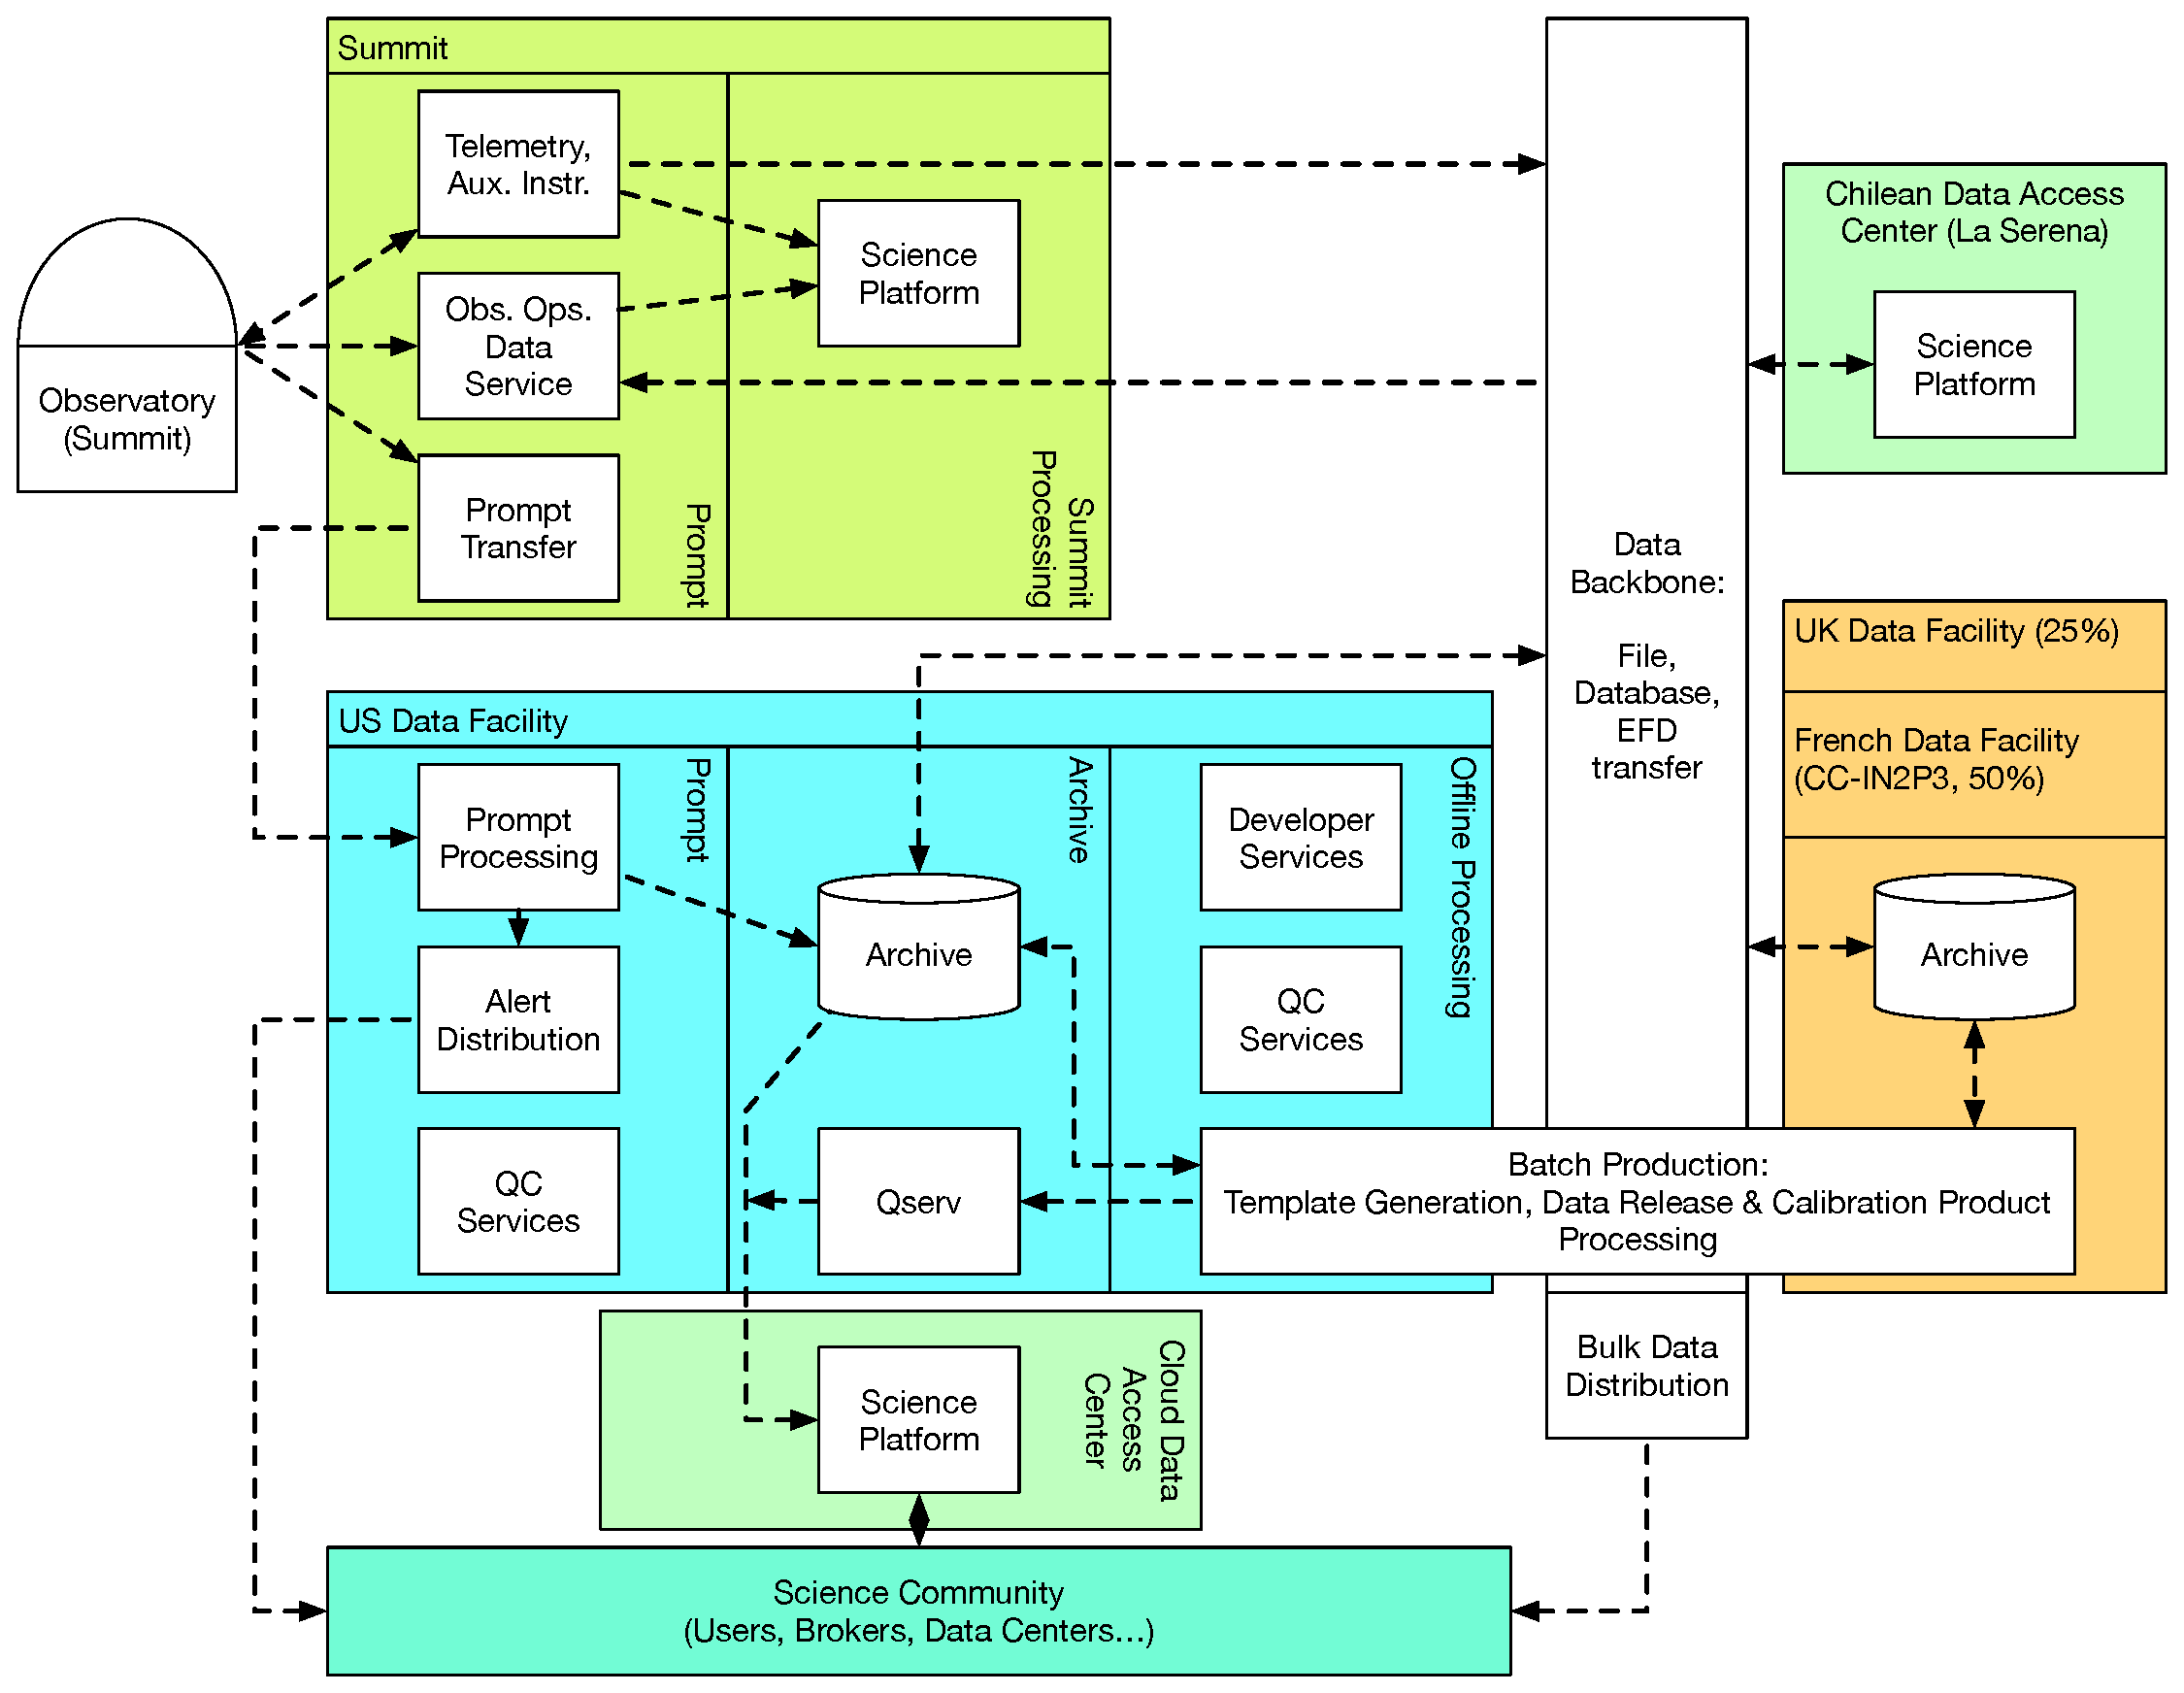
\includegraphics[width=\textwidth]{I08_f1.eps }
	\caption{ Simplified  Vera C. Rubin Architecture diagram from Magic Draw \label{fig:arch}}
\end{centering}
\end{figure}

\subsection{Data Release Processing}\label{sec:DRP}
\subsection{Prompt Processing} \label{sec:prompt}


\section{Lessons learned}
Some of the software best practices are given in \citet{2018SPIE10707E..09J}.

\bibliography{I08}
\end{document}
